\documentclass{article}
\usepackage[T1]{fontenc}
\usepackage[utf8]{inputenc}
\usepackage[margin=1in]{geometry}
\usepackage{booktabs}
\usepackage{graphicx}
\usepackage{xcolor}
\usepackage{tikz}
\usetikzlibrary{arrows.meta,positioning,shapes.geometric,fit,calc}
\usepackage[hidelinks]{hyperref}

\newcommand{\code}[1]{\texttt{#1}}

\tikzset{
  block/.style={
    rectangle,
    rounded corners,
    draw=blue!65!black,
    fill=blue!7,
    align=center,
    minimum width=2.8cm,
    minimum height=0.9cm,
    font=\small
  },
  store/.style={
    cylinder,
    shape border rotate=90,
    draw=teal!70!black,
    fill=teal!8,
    align=center,
    aspect=0.25,
    minimum width=2.8cm,
    minimum height=1.0cm,
    font=\small
  },
  risk/.style={
    rectangle,
    rounded corners,
    draw=red!70!black,
    fill=red!7,
    align=center,
    minimum width=3.0cm,
    minimum height=0.9cm,
    font=\small
  },
  decision/.style={
    diamond,
    draw=orange!80!black,
    fill=orange!10,
    align=center,
    aspect=1.8,
    font=\small
  },
  arrow/.style={-{Latex[length=2.5mm]}, thick},
  dashedarrow/.style={-{Latex[length=2.5mm]}, thick, dashed}
}

\begin{document}

\title{The Right to Erasure, Sensitive Metadata Accumulation, and Device-Aware Video Anonymization in Medical Data}
\author{Thomas J. Lux, Max Hild, SM Hamza Zahid}
\date{February 2026}
\maketitle

\begin{abstract}
Endoscopic video and reports routinely contain patient-identifying overlays,
operator identifiers, timestamps, case identifiers, and institutional metadata.
These data are useful during care but unsafe for secondary use without governed
de-identification. GDPR Article 17 codifies a right to erasure, which motivates
storage, deletion, and de-identification controls across the anonymization
lifecycle. \cite{gdpr} This paper presents an implementation-oriented workflow
for endoscopy environments based on three linked elements: sampled-frame
sensitive metadata accumulation, processor-aware anonymization of video output,
and pseudonymized linkage for grouping records without exposing direct
identifiers. Hashing is treated as a linkage and governance mechanism, not as a
standalone guarantee of anonymity. The workflow is designed for real clinical
infrastructure where overlay geometry, rendering style, device family, and data
density differ substantially.
\end{abstract}

\section{Clinical Motivation}
Modern endoscopy systems superimpose textual and symbolic information directly
onto the live image stream. These overlays often include patient name elements,
date of birth, accession or case identifiers, examination date and time,
examiner identity, and center labels. In routine clinical operation, these
fields support workflow continuity and medico-legal traceability. For quality
improvement, education, AI development, and multicenter research, retaining
such information creates substantial privacy and governance risk.

The management and sharing of healthcare data for research purposes present
significant challenges in security, privacy, and regulatory compliance,
particularly under frameworks such as HIPAA and GDPR.
\cite{barbaria2025advancing}\cite{prakaashana2025measuring} Facilitating data
sharing and harmonization for multicenter collaborations becomes especially
difficult when protected health information (PHI) is embedded directly within
image pixels. Recent reviews on burnt-in text recognition in medical imaging
describe problems caused by low resolution, compression artifacts, motion blur,
and background interference. \cite{osagie2024burnt}

The central clinical challenge is therefore not merely to remove text, but to
reduce identifying context while preserving mucosal findings, instrument
position, and procedure dynamics.

\section{Conceptual Framework}
\subsection{Sensitive Metadata Accumulation}
Sensitive metadata accumulation integrates evidence from many sampled frames
into a patient- and procedure-level representation. Single-frame OCR often
produces incomplete fragments because overlays may be transient, blurred,
partially occluded, or rendered with changing contrast. A practical system must
therefore merge partial detections over time, preserve high-confidence fields,
and expose uncertainty for validation rather than silently treating missing
fields as proof of safety.

This temporal accumulation model improves robustness in two ways:
\begin{itemize}
  \item it reduces dependence on any single frame;
  \item it supports earlier identification of critical identifiers even when no
  single frame contains the complete demographic block.
\end{itemize}

\subsection{Device-Aware Anonymized Video Return}
Endoscopy platforms differ in overlay placement, viewport geometry, metadata
panel structure, and rendering style. A single fixed anonymization mask is
therefore rarely safe across device families. Device-aware anonymization uses
processor-specific region-of-interest (ROI) definitions to preserve the
endoscopic image viewport while suppressing side panels, banners, or other
regions where identifying metadata is expected.

In the implemented workflow, the processor configuration supplies ROI metadata
to the anonymization step. The anonymizer then applies either viewport-preserving
masking or frame-level suppression depending on local policy and the detected
content. This produces an output video intended to remain clinically
interpretable, but it still requires validation before release.

\subsection{Pseudonymized Linkage Is Not Anonymity}
The workflow uses deterministic hashes to group related records and examinations
without exposing direct identifiers. This supports longitudinal review and
report/video linkage, but pseudonymization is not equivalent to anonymization.
If the input attributes, salt, or linkage context are known, deterministic
hashes can remain personal data under GDPR. Consequently, hashes should be
described as controlled linkage identifiers and protected by key, salt, access,
and audit policy.

\section{Implementation Workflow}
In a real endoscopy environment, anonymization must operate under practical
constraints:
\begin{itemize}
  \item heterogeneous videos and reports from different rooms and vendors;
  \item variable codec quality, frame rate, and overlay persistence;
  \item need for reproducible import, processing, validation, and audit;
  \item storage requirements where canonical media may be encrypted at rest.
\end{itemize}

Figure~\ref{fig:pipeline} shows the intended workflow. The canonical stored
object is the encrypted Django \code{FileField}. External tools that require a
filesystem path receive a local plaintext working copy. Optional streamable
artifacts are generated only for protected media delivery paths.

\begin{figure}[htbp]
\centering
\resizebox{\textwidth}{!}{%
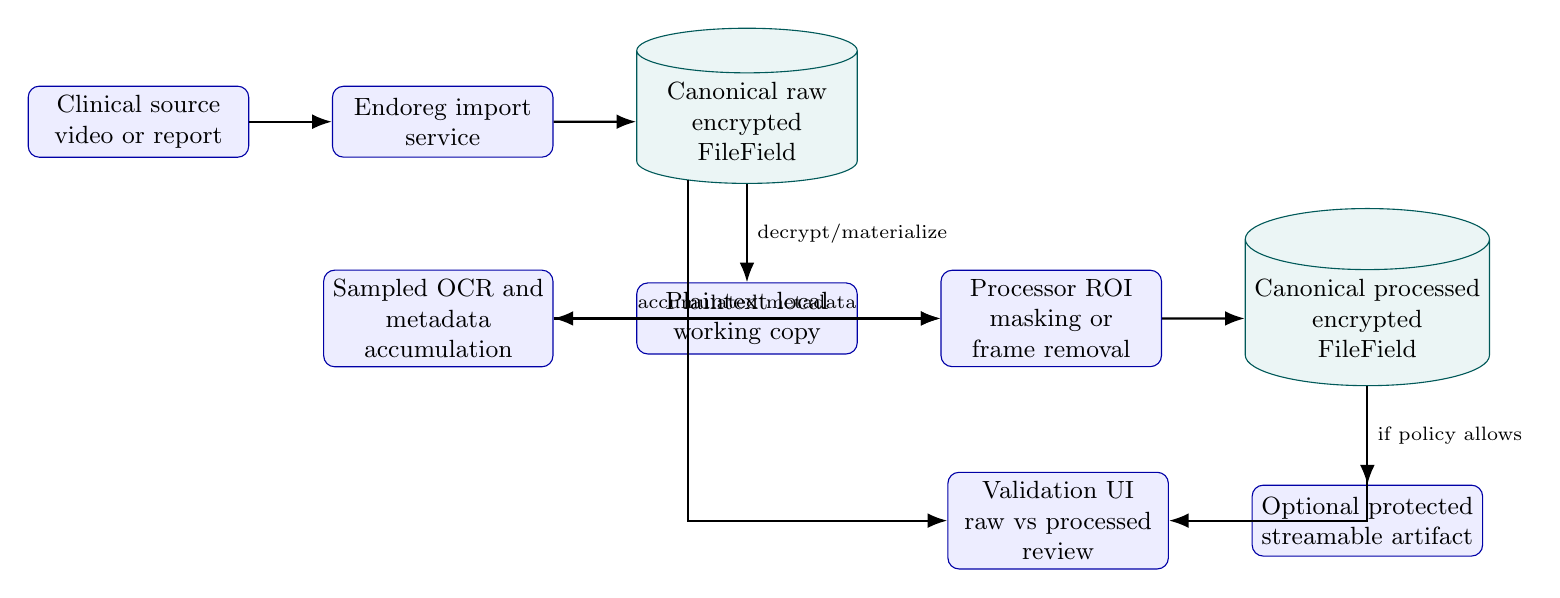
\begin{tikzpicture}[node distance=1.25cm and 1.05cm]
  \node[block] (source) {Clinical source\\video or report};
  \node[block, right=of source] (import) {Endoreg import\\service};
  \node[store, right=of import] (raw) {Canonical raw\\encrypted\\FileField};
  \node[block, below=of raw] (materialize) {Plaintext local\\working copy};
  \node[block, left=of materialize] (analysis) {Sampled OCR and\\metadata\\accumulation};
  \node[block, right=of materialize] (roi) {Processor ROI\\masking or\\frame removal};
  \node[store, right=of roi] (processed) {Canonical processed\\encrypted\\FileField};
  \node[block, below=of processed] (streamable) {Optional protected\\streamable artifact};
  \node[block, left=of streamable] (validation) {Validation UI\\raw vs processed\\review};

  \draw[arrow] (source) -- (import);
  \draw[arrow] (import) -- (raw);
  \draw[arrow] (raw) -- node[right,font=\scriptsize] {decrypt/materialize} (materialize);
  \draw[arrow] (materialize) -- (analysis);
  \draw[arrow] (analysis) -- node[above,font=\scriptsize] {accumulated metadata} (roi);
  \draw[arrow] (materialize) -- (roi);
  \draw[arrow] (roi) -- (processed);
  \draw[dashedarrow] (processed) -- node[right,font=\scriptsize] {if policy allows} (streamable);
  \draw[arrow] (raw.south west) |- (validation.west);
  \draw[arrow] (processed.south) |- (validation.east);
\end{tikzpicture}}
\caption{Implementation workflow for encrypted canonical storage, local
plaintext processing, optional protected streamable artifacts, and human
validation.}
\label{fig:pipeline}
\end{figure}

\section{Clinical Relevance of Accumulated Metadata}
Accumulated metadata serves three clinical and governance functions beyond
redaction itself:
\begin{enumerate}
  \item \textbf{Verification:} it records whether known identifying fields were
  detected in the source material.
  \item \textbf{Auditability:} it provides structured evidence for privacy
  review and release decisions.
  \item \textbf{Context preservation:} it allows retention of non-identifying
  procedure descriptors where policy permits.
\end{enumerate}

The goal is not to claim that every identifier has been removed automatically.
The goal is to reduce re-identification risk and make residual risk visible
enough for governed validation.

\section{Device-Specific Anonymization Strategies}
Two strategy families are clinically relevant:
\begin{itemize}
  \item \textbf{Mask-based viewport preservation:} preserve the endoscopic
  image region and suppress surrounding metadata zones according to processor
  geometry.
  \item \textbf{Frame-level suppression or removal:} remove or transform frames
  judged to contain high-risk identifying overlays.
\end{itemize}

Device-aware selection between these strategies should be guided by local
policy, research protocol, and downstream use. For teaching archives, viewport
preservation may maximize clinical value. For strict secondary-use contexts,
more aggressive frame suppression may be appropriate.

\section{Processing Defaults}
During import and the first anonymization pass, the video workflow uses
sampled-frame OCR and metadata extraction. The current video path preferentially
uses TesserOCR when available and falls back to PyTesseract for compatibility.
\cite{tesserocr2018}\cite{smith2007overview} The broader image and report
pipeline can combine text detection and OCR components such as EAST,
Tesseract-based detection, and additional OCR engines where configured.
\cite{ZERONE2024}\cite{Ribeiro2019OCRcompare}

For clarity, these are implementation defaults rather than safety guarantees.
Performance-oriented choices must be evaluated separately from privacy safety:
faster OCR is useful only if identifier recall remains acceptable under the
local release policy.

\section{Validation Interface and Human Review}
The validation interface supports direct comparison of raw and processed media
for authorized users. For video, raw and anonymized streams can be displayed
side by side, synchronized during playback, and reviewed together with segment
annotations. For reports, raw and anonymized PDFs can be compared in the same
review context.

This interface is essential because automated detection is probabilistic.
Approval should therefore depend on both metadata validation and visual review.
The ``outside'' label describes video segments acquired outside the patient's
body or otherwise unsuitable for downstream clinical analysis. Such segments can
be presented to reviewers for confirmation before they are removed, censored, or
excluded from derived datasets.

\section{Safety, Limitations, and Governance}
Despite practical utility, several limitations remain clinically important:
\begin{itemize}
  \item transient identifiers may be missed under sparse sampling;
  \item overlay drift after firmware updates can invalidate ROI assumptions;
  \item OCR uncertainty in low-quality captures can propagate into incomplete
  metadata accumulation;
  \item pseudonymized hashes support linkage but do not by themselves satisfy
  anonymization.
\end{itemize}

Endoscopy anonymization should therefore be treated as a governed clinical
process rather than a one-time technical transform. Recommended safeguards
include validation on local device output, periodic ROI review after firmware
or hardware changes, privacy-officer review of release policy, and predefined
identifier recall criteria before secondary use.

\section{Implications for Medical AI and Research}
A reliable accumulation-plus-device-awareness model supports safer scaling of
endoscopy data use in three domains:
\begin{itemize}
  \item multicenter dataset construction with reduced privacy risk;
  \item quality improvement programs using longitudinal video review;
  \item AI model development on de-identified yet clinically useful visual data.
\end{itemize}

Foundational papers on medical AI emphasize that data lacking in volume,
diversity, and annotation produce limited generalization.
\cite{moor2023foundation} The lack of freely distributable health records has
long hindered healthcare innovation. \cite{walonoski2018synthea} Creating
AI-ready datasets from surgical and endoscopic video relies heavily on careful
de-identification. \cite{bilal2025temset}

The contribution of the workflow is operational trust: clinicians and
governance teams can inspect why a video was considered releasable, which
metadata signals were detected, and which device-specific masking strategy was
used.

\section{Evaluation Plan}
The current evidence should be reported as an evaluation plan unless measured
results are available. A complete evaluation should compare the proposed
workflow against a single-frame OCR baseline, a fixed-mask baseline, and a
conservative full-banner suppression baseline.

\begin{table}[htbp]
\centering
\begin{tabular}{p{0.28\textwidth}p{0.58\textwidth}}
\toprule
\textbf{Metric} & \textbf{Purpose} \\
\midrule
Frame-level PHI leakage & Counts a frame as unsafe if any ground-truth PHI
entity is not sufficiently covered or removed. \\
Viewport preservation ratio & Measures how much diagnostically relevant
endoscopic viewport remains visible after anonymization. \\
OCR field recall & Measures whether patient name, date of birth, case number,
examiner, date/time, and institution fields are detected. \\
Review burden & Measures how many cases require manual correction, segment
validation, or exclusion. \\
Runtime and resource use & Measures total import time, anonymizer time,
throughput, CPU time, and memory use. \\
\bottomrule
\end{tabular}
\caption{Evaluation dimensions needed before making strong clinical safety
claims.}
\label{tab:evaluation}
\end{table}

Historically, approaches to burned-in text have involved either removing all
burned-in text regardless of content, which can discard valuable clinical
markers, or applying heuristic rules that struggle to generalize to new PHI
formats. \cite{macdonald2024method} Device-aware viewport preservation addresses
this trade-off by preserving diagnostic content while redacting expected PHI
regions. Recent evaluations of vision-language models also caution that simple
spatial masking does not automatically prevent PHI leakage, because structured
identifiers may still be inferred from context. \cite{young2025vision}

\section{Deleting Records Safely}
Safe deletion in endoscopy anonymization is a controlled clinical workflow, not
a single database action. Deletion should combine transaction boundaries,
storage-aware file removal, scoped annotation cleanup, and durable operation
logs. Importantly, the right to erasure should not be confused with
pseudonymization: a hash may preserve linkage even after direct identifiers are
removed.

\begin{figure}[htbp]
\centering
\resizebox{\textwidth}{!}{%
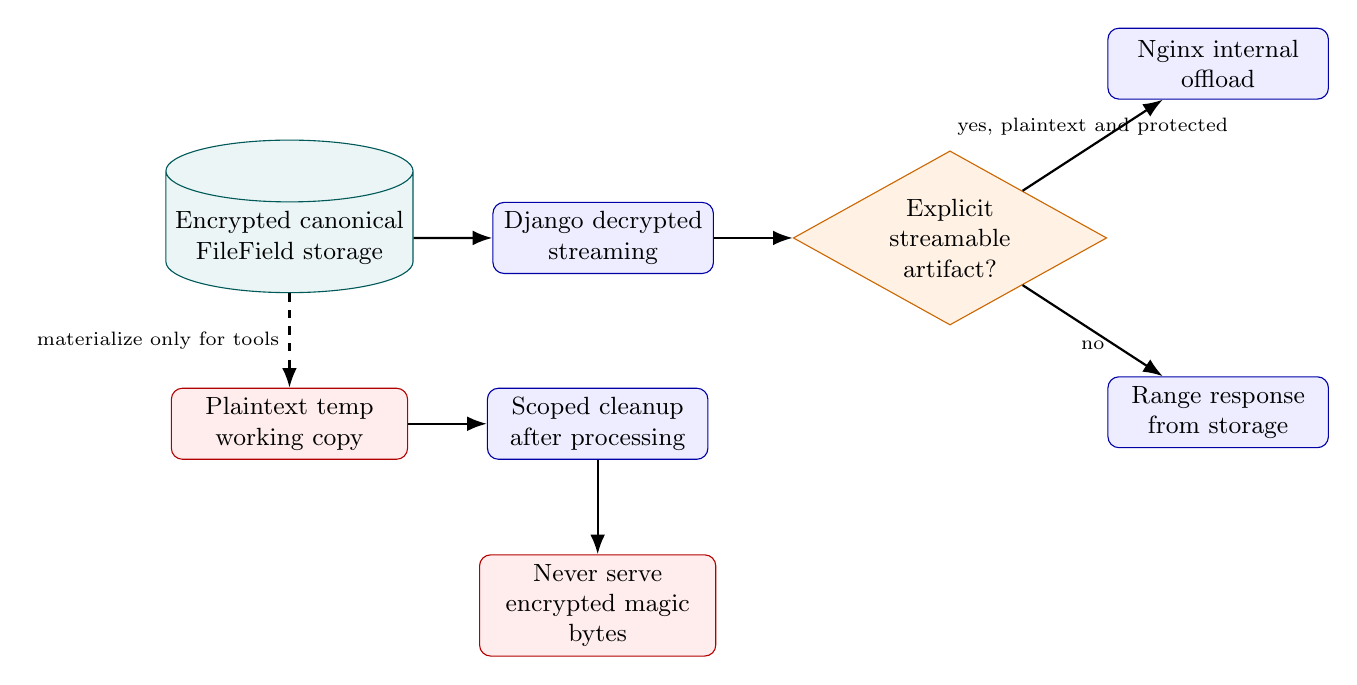
\begin{tikzpicture}[node distance=1.2cm and 1.0cm]
  \node[store] (canonical) {Encrypted canonical\\FileField storage};
  \node[block, right=of canonical] (stream) {Django decrypted\\streaming};
  \node[decision, right=of stream] (nginx) {Explicit\\streamable\\artifact?};
  \node[block, above right=of nginx] (accel) {Nginx internal\\offload};
  \node[block, below right=of nginx] (django) {Range response\\from storage};
  \node[risk, below=of canonical] (temp) {Plaintext temp\\working copy};
  \node[block, right=of temp] (cleanup) {Scoped cleanup\\after processing};
  \node[risk, below=of cleanup] (deny) {Never serve\\encrypted magic\\bytes};

  \draw[arrow] (canonical) -- (stream);
  \draw[arrow] (stream) -- (nginx);
  \draw[arrow] (nginx) -- node[above,font=\scriptsize] {yes, plaintext and protected} (accel);
  \draw[arrow] (nginx) -- node[below,font=\scriptsize] {no} (django);
  \draw[dashedarrow] (canonical) -- node[left,font=\scriptsize] {materialize only for tools} (temp);
  \draw[arrow] (temp) -- (cleanup);
  \draw[arrow] (cleanup) -- (deny);
\end{tikzpicture}}
\caption{Storage and streaming boundary. Canonical files remain encrypted at
rest. Plaintext exists only as local working copies or explicit protected
streamable artifacts.}
\label{fig:storage-boundary}
\end{figure}

\subsection{Operational Principles}
\begin{itemize}
  \item \textbf{Use atomic units of work:} related metadata updates, annotation
  cleanup, and parent-record state transitions should commit or roll back
  together.
  \item \textbf{Delete by scope:} frame-level annotation deletion must be
  constrained by video, frame range, label, source, and provenance.
  \item \textbf{Keep a durable audit trail:} destructive operations should log
  resource type, identifier, actor, reason, and before/after status.
  \item \textbf{Prefer idempotent cleanup:} repeated deletion requests should
  converge to the same safe state.
\end{itemize}

\subsection{Clinical Safety Guardrails}
\begin{itemize}
  \item \textbf{Separate validation from deletion:} review workflows and
  destructive actions should not be conflated.
  \item \textbf{Gate hard deletion by policy:} sensitive records should pass
  role-based, retention, and governance checks before irreversible removal.
  \item \textbf{Verify after deletion:} safety checks should confirm that no
  orphaned annotations, plaintext temporary files, or inconsistent state records
  remain.
\end{itemize}

\section{Conclusion}
Effective endoscopy de-identification requires temporal evidence, device
context, storage-aware implementation, and governed human validation. Sensitive
metadata accumulation improves robustness over single-frame analysis, while
processor-aware masking helps preserve diagnostic content. Pseudonymized hashes
support record linkage but do not replace anonymization or deletion policy.
Together, these principles move de-identification from a narrow image-processing
task toward a clinically governed lifecycle for secondary use of endoscopic
video and report data.

\newpage
\bibliographystyle{plain}
\bibliography{bib}

\end{document}
